% !TEX TS-program = LuaLaTeX
\documentclass[10pt, oneside, a4paper]{article}

\usepackage[T1]{fontenc}
\usepackage{lmodern}
\usepackage{xcolor}
    \definecolor{gray} {HTML}{363636}
    \definecolor{red}  {HTML}{950009}
    \definecolor{green}{HTML}{0E610A}
    \definecolor{blue} {HTML}{020069}
    \definecolor{bglst}{HTML}{F4F4F4}
\usepackage{fontspec}
    \setsansfont{Arial}
\usepackage{amsmath}
\usepackage{titlesec}
    \titleformat*{\section}      {\color{gray}\large\bfseries\sffamily}
    \titleformat*{\subsection}   {\color{gray}\large\bfseries\sffamily}
    \titleformat*{\subsubsection}{\color{gray}\large\bfseries\sffamily}
\usepackage{geometry}
    \geometry{scale={0.75,0.85}}
\usepackage{siunitx}
    \sisetup{locale=FR}
\usepackage{graphicx}
\usepackage{caption}
    \captionsetup{labelfont={bf,sf,color=gray}}
\usepackage{pdfpages}
\usepackage{minted}
    \setminted{linenos}
    \setminted{fontsize=\footnotesize}
    \setminted{bgcolor=bglst}
    \setminted{style=borland}
\usepackage{enumitem}

% Keep lasts
\usepackage[french]{babel}
    \frenchsetup{SmallCapsFigTabCaptions=false}
\usepackage[expansion]{microtype}
\usepackage[luatex, backref]{hyperref}
    \hypersetup{unicode, colorlinks, breaklinks, urlcolor=red,
                bookmarksopen, bookmarksnumbered}

\renewcommand{\UrlFont}{\small}
\renewcommand{\arraystretch}{1.1}
\newcommand{\important}[1]{\textbf{\textsf{\color{gray}{#1}}}}
\setlength{\parskip}{8pt}

\begin{document}

\begin{titlepage}
    \centering
    
\includegraphics[width=0.5\textwidth]{images/logo-ecam.png}\par
    \vspace{1cm}

    \rule{\linewidth}{1.5pt}%
    \vspace{5mm}
    {\rm\sffamily\LARGE Techniques de transmission et traitement du signal\par}
    \vspace{3mm}
    {\sffamily\bfseries\LARGE Simulation d’une chaîne de transmission\\
                              numérique avec MATLAB\textregistered{}\par}
    \vspace{5mm}
    \rule{\linewidth}{1.5pt}%
    \vspace{1cm}

    {\large%
        \begin{minipage}[t]{0.35\linewidth}
            \centering
            Alexis~\bsc{Nootens} \\[1mm]
            \href{mailto:16139@student.ecam.be}{16139@student.ecam.be}
        \end{minipage}
        \begin{minipage}[t]{0.35\linewidth}
            \centering
            Armen~\bsc{Hagopian} \\[1mm]
            \href{mailto:14040@student.ecam.be}{14040@student.ecam.be}
        \end{minipage}
    \par}
    \vspace{1cm}

    {\large%
        ECAM Brussels             \\[1mm]
        Promenade de l'Alma 50    \\[1mm]
        1200 Woluwe-Saint-Lambert \\[1mm]
        Belgique
    \par}

    \vfill
    {\large\today\par}
\end{titlepage}

%%%%%%%%%%%%%%%%
\tableofcontents
\newpage

%%%%%%%%%%%%%%%%%%%%%%%
\phantomsection
\section*{Introduction}
\addcontentsline{toc}{section}{Introduction}
L'objectif de ce projet est de simuler la couche physique d'un protocole de communication, c'est-à-dire le niveau 1 du modèle OSI.
La simulation est réalisée à l'aide du logiciel MATLAB\textregistered{} édité par Mathworks\textregistered{}.
Une contrainte imposée dans la simulation est de tenir compte de plusieurs émetteurs et receveurs pouvant communiquer simultanément.
Pour répondre à cette contrainte, la couche physique implémentée utilise le multiplexage fréquentiel.

Ce document reprend la conception du projet et les choix qui ont dû y être décidés, accompagnés de leur explication.


%%%%%%%%%%%%%%%%%%%%%%%%
\section{Implémentation}
\label{sec:implementation}
La section~\ref{sec:implementation} décrit le modus operandi réalisé dans les fichiers qui composent le projet.
Ces fichiers peuvent être consultés à l'annexe~\ref{sec:fichiers-sources}.
Ils consistent en :
\begin{description}[align=right,labelwidth=2cm,labelindent=1cm]
    \item[main.m] lance les scripts dans l'ordre logique.
    \item[parameters.m] configure paramètres de simulation.
    \item[sender.m] génère les données aléatoirement, puis sépare les canaux
        fréquentiellement.
    \item[channel.m] simule un canal de communication en atténuant et filtrant les signaux.
    \item[receiver.m] démodule les signaux reçus et tente de recomposer le signal émis.
\end{description}

\subsection{Fichier principale}
Le fichier principal, nommé \texttt{main.m} par son nom anglais et consultable à l'annexe~\ref{app:main}, se charge principalement de lancer les scripts composants la simulation dans un ordre logique.
Son contenu est minime, il commence par nettoyer le plan de travail des variables et figures résiduelles.
Il lance ensuite les scripts dans l'ordre : \texttt{parameters.m} $\rightarrow$ \texttt{sender.m} $\rightarrow$ \texttt{channel.m} $\rightarrow$ \texttt{receiver.m}.

Une fois la simulation terminée, il affiche également une figure comparant le signal dans un canal émis par l'émetteur, au signal recomposé dans ce même canal par le receveur.
La figure~\ref{fig:comparaison} présente un exemple de cette comparaison.
On peut y apercevoir que le signal recomposé est délayé par rapport au signal émis, et que ses amplitudes aux pics isolés sont quasiment divisées par deux.
Cela est normal étant donné que l'on retrouve plus de fréquence dans un pic isolé que dans une succession à la même amplitude.
Ce pic souffrira donc plus fortement au filtrage fréquentiel.

\begin{figure}[p]
    \centering
    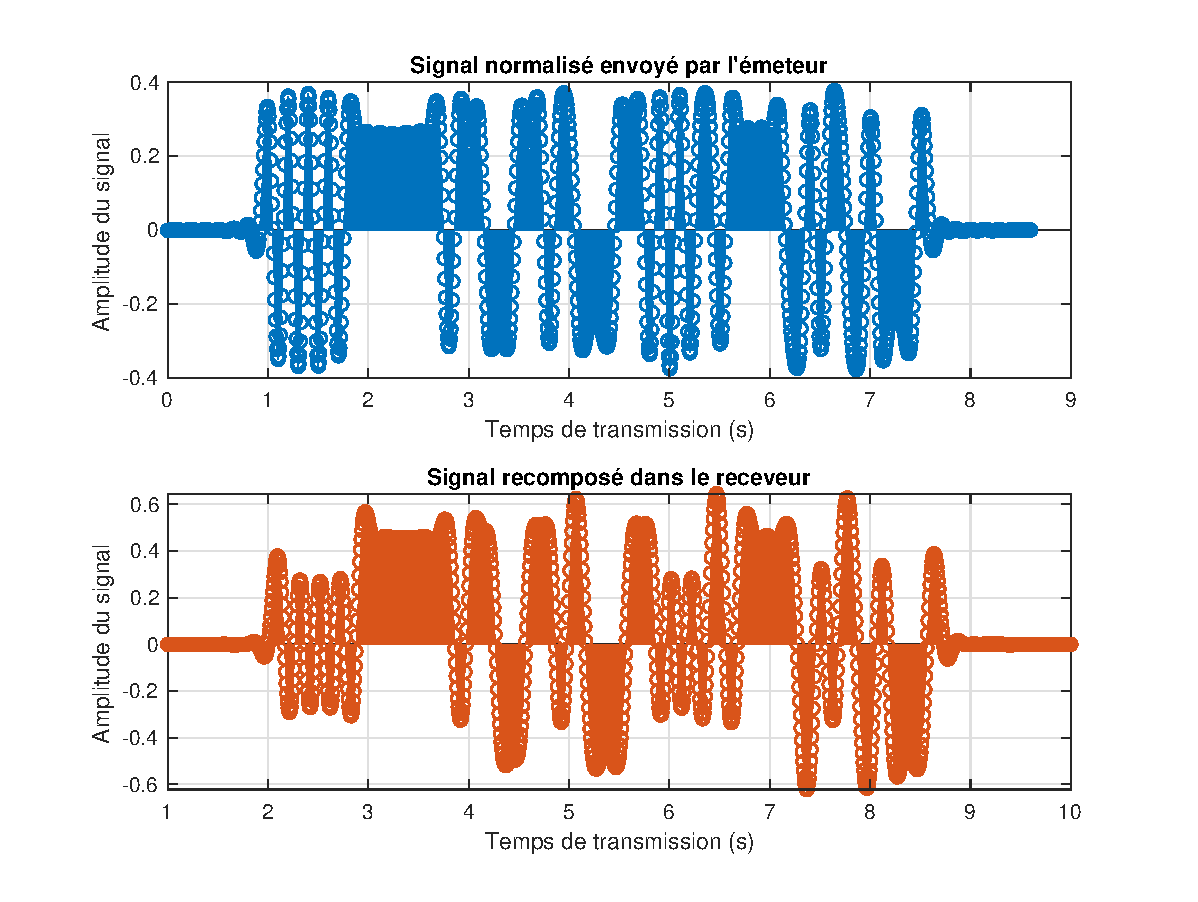
\includegraphics[height=0.45\textheight]{eps/comparaison.eps}
    \caption{Comparaison entre le signal en bande de base émis dans l'émetteur et celui
             recomposé dans le receveur.
             Le signal reçu est décalé d'approximativement 1 seconde par rapport au signal
             émis.
             Le signal reçu est également plus sévèrement atténué aux pics isolés qui
             contiennent des plus hautes fréquences.
             Le rapport d'amplitude n'est pas conservé car le receveur ne tente pas de
             compenser la perte de tension dans le canal.
             À la place le signal est juste normalisé à \SI{200}{\milli\watt} avant
             d'être émis.}
    \label{fig:comparaison}
\end{figure}

\subsection{Paramètres}
Le fichier \texttt{parameters.m}, consultable à l'annexe~\ref{app:paremeters}, offre un accès rapide et concentré aux différents paramètres influençant la simulation tel que la quantité de canaux fréquentiels disponibles, la taille du message à envoyer, ou encore la vitesse d'envoi.
Chaque paramètre est accompagné d'un commentaire expliquant dûment son utilité.

\subsection{Émetteur}
Le fichier \texttt{emetteur.m}, consultable à l'annexe~\ref{app:sender}, commence la simulation proprement dite.
Il débute par générer une séquence de bits aléatoires suivant une distribution normale grâce à \mintinline{matlab}{randn()}.

\subsubsection{Séquence de départ}
Il rajoute une séquence de départ pour la forme uniquement.
Cette dernière n'est pas exploitée dans le receveur, mais trouve son utilité dans l'appréciation qualitative du canal par nos yeux.
Cette séquence consiste premièrement en 4 oscillations de symboles opposés $(1,0,1,0,1,0,1,0)$, puis de 8 symboles identiques $(1,1,1,1,1,1,1,1)$.
L'intérêt de cette séquence est de constater la réponse du canal aux plus hautes fréquences du signal, et l'amplitude RMS d'un message constant.
Cette séquence de départ est aisément distinguable à la figure~\ref{fig:comparaison}.

Après l'ajout de la séquence de départ, les bits sont codés dans un code PAM-2 où les 0 deviennent $-1$ et les 1 restent 1.

\subsubsection{Cosinus surélevé}
Afin de diviser le spectre fréquentiel pour y définir des canaux, il faut s'assurer que les messages envoyés se limitent à leur bande allouée.
Pour ce faire nous pouvons utiliser le filtre en sinus cardinal qui à la merveilleuse propriété que pour un signal avec une durée de symbole de $T_b$ secondes, il ne consommera que $\frac{1}{2T_b}$ largeur de spectre dans le domaine fréquentiel.
C'est mathématiquement la meilleure efficacité spectrale atteignable.

Un soucis survient avec l'utilisation de ce filtre en pratique, c'est que le signal codé maintient son amplitude maximale, dénommée plafond, durant un bref instant puis chute brusquement.
Ce type de réponse n'est pas utilisable en pratique car la fréquence de capture d'échantillons dans le receveur n'est ni monotone, ni même en phase.
Pour adresser ce problème, nous utilisons une version alternative du sinus cardinal nommée le filtre en cosinus surélevé.
Ce filtre a la particularité de maintenir son plafond plus longtemps, mais aux prix de flancs montants et descendants plus raides car la période d'expression d'un symbole n'est pas augmentée.
Ces flancs plus raides entrainent une plus grande consommation de bande spectrale.
Le cosinus surélevé définit une largeur de bande consommée $1+\alpha$ avec \alpha{} dénommé \og{}facteur de roll-off\fg{} compris dans l'intervalle $0\leq\alpha\leq1$.
Un $\alpha = 0$ rend le filtre égale à celui d'un sinus cardinal.
Ce facteur contrôle le temps de plafond d'un symbole dans le domaine temporel.
Dans notre implémentation, nous avons choisi un facteur $\alpha = \num{0.4}$ arbitrairement.

\subsubsection{Sur-échantillonnage}
La description du filtre précédemment faite s'applique au domaine continu.
Quand nous passons dans le domaine discret, le temps d'échantillonnage doit être pris en compte.
Si nous n'utilisons qu'un seul échantillon pour convoluer le filtre en cosinus surélevé, sa réponse impulsionnelle sera semblable à une impulsion de Dirac, avec une consommation fréquentielle infinie, ce qui est l'opposé de ce qui est désiré.
Et si nous utilisons une infinité d'échantillons, nous obtiendrons une réponse parfaite semblable au domaine continue.
Connaissant les extrémités, nous nous intéressons à savoir combien d'échantillons au minimum sont nécessaires pour garder les spectres de différents canaux séparés.
L'équation~(\ref{eqn:calcule-de-beta-final}) répond à cette question.
En partant de l'équation~(\ref{eqn:calcule-de-beta-initial}) qui fixe les contraintes.

Soit $T_n$ le taux d'échantillonnage nécessaire pour restreindre les canaux à leur bande sans qu'ils ne s'empiètent, $T_b$ le taux d'échantillonnage du signal avant filtrage, $N$ le nombre de canaux actifs et \alpha{} le facteur de roll-off.
Puisque le premier canal non-modulé sera \og{}single-sideband\fg{} $\frac{1}{2T_b}$, et les suivants seront \og{}double-sideband\fg{} $\frac{1}{T_b}$ :
\begin{align}
\intertext{Par le théorème de Nyquist} 
\frac{1}{2T_n}      &\geq \left[ \frac{1}{2T_b} + \left( N-1 \right) \frac{1}{T_b} \right] \left( 1 + \alpha \right)
\label{eqn:calcule-de-beta-initial}\\[2mm]
\intertext{Puisque \beta{} est le rapport $T_n \div T_b$} 
\frac{\beta}{2T_b}  &\geq \left[ \frac{1}{2T_b} + \left( N-1 \right) \frac{1}{T_b} \right] \left( 1 + \alpha \right) \\[2mm]
\intertext{En rajoutant $2T_b$ de chaque côté} 
\beta               &\geq \Big[ 1 + \left( N-1 \right) 2 \Big] \left( 1 + \alpha \right) \\[2mm]
\intertext{En considérant le pire cas de $\alpha = 1$} 
\beta               &\geq 2 + \left( N-1 \right) 4 \\[2mm]
\intertext{En simplifiant}
\beta               &\geq 4N - 2
\label{eqn:calcule-de-beta-final}
\end{align}
Et puisque nous n'aimons pas ce qui n'est pas linéaire, nous prenons dans la simulation $\beta = 4N$.

Un dernier paramètre à décider dans la construction du filtre numérique est la longueur de la réponse impulsionnelle qui va servir à convoluer le signal.
Pour que le filtrage respecte parfaitement les caractéristiques que nous lui avons défini, il lui faut une longueur infinie.
Ceci n'étant pas possible en pratique, la réponse doit être tronquée tout en gardant le maximum de puissance.
Par essaies empiriques, nous avons déterminé que 20 fois le taux de sur-échantillonnage est une bonne valeur.

\subsubsection{Modulation}
Les filtres générés et leurs réponses impulsionnelles obtenues, nous les modulons par les porteuses avant d'être convolués avec le signal.
Les fréquences des porteuses sont obtenues en séparant chaque canal par $\frac{1}{2Tb}$
Nous obtenons les impulsions présentées à la figure~\ref{fig:impulse}.
Cette figure présente les 3 impulsions nécessaires pour multiplexer en 3 canaux.
Il est intéressant de constater que l'impulsion du canal 2 est inversée en amplitude.

\begin{figure}[p]
    \centering
    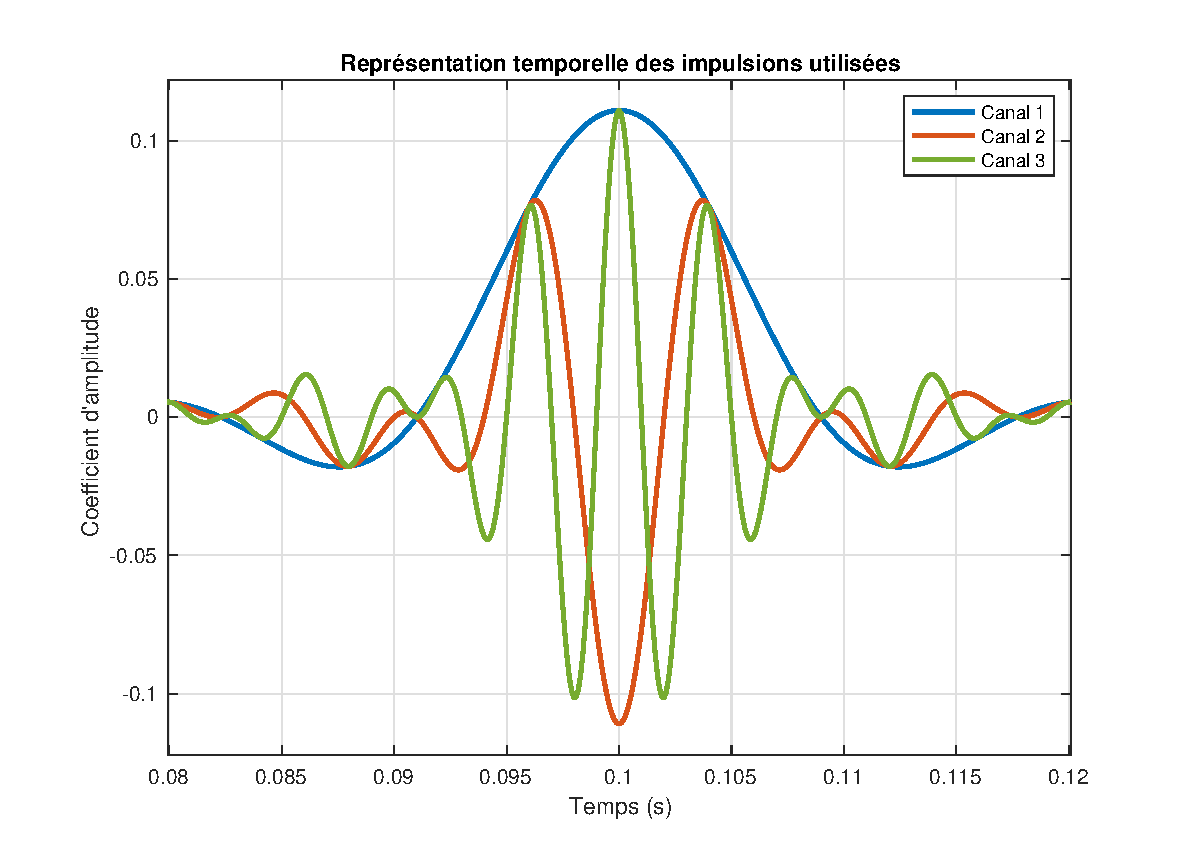
\includegraphics[height=0.4\textheight]{eps/impulse.eps}
    \caption{Représentation temporelle des impulsions utilisées pour multiplexer en 3 canaux.
             Chaque des impulsions est sa réponse en bande de base modulée par sa porteuse.
             Il est intéressant de constater que l'impulsion du canal 2 est inversée en
             amplitude.}
    \label{fig:impulse}
\end{figure}

Les signaux modulés, leur puissance est normalisée à une quantité de milliwatt en multipliant les amplitudes par le facteur adéquat.
Nous normalisons la puissance du signal après la modulation car la puissance de la porteuse s'additionne au signal utile.
Si nous le faisions avant, nous retrouverions une puissance deux fois plus grande dans le premier canal, sans porteuse, que dans les autres.
La puissance de chaque canal est évaluée en intégrant la norme au carré sur l'impédance caractéristique du milieu de propagation.
Dans notre simulation, nous avons choisi d'évaluer la puissance par $Z_0 = \SI{1}{\Omega}$ et nous normalisons à \SI{200}{\milli\watt}.

\begin{equation}
    P[s] = \frac{\frac{1}{N} \sum_{n = 0}^{N} s[n]^2}{Z_0}
\end{equation}

Le script \texttt{sender.m} affiche un récapitulatif de la transmission en temporel et fréquentiel avant de sommer tous les canaux pour les envoyer sur le seul lien physique disponible, le cable ou le rayonnement électromagnétique.
Un exemple de ce récapitulatif est présenté à la figure~\ref{fig:sender}.

\begin{figure}[p]
    \centering
    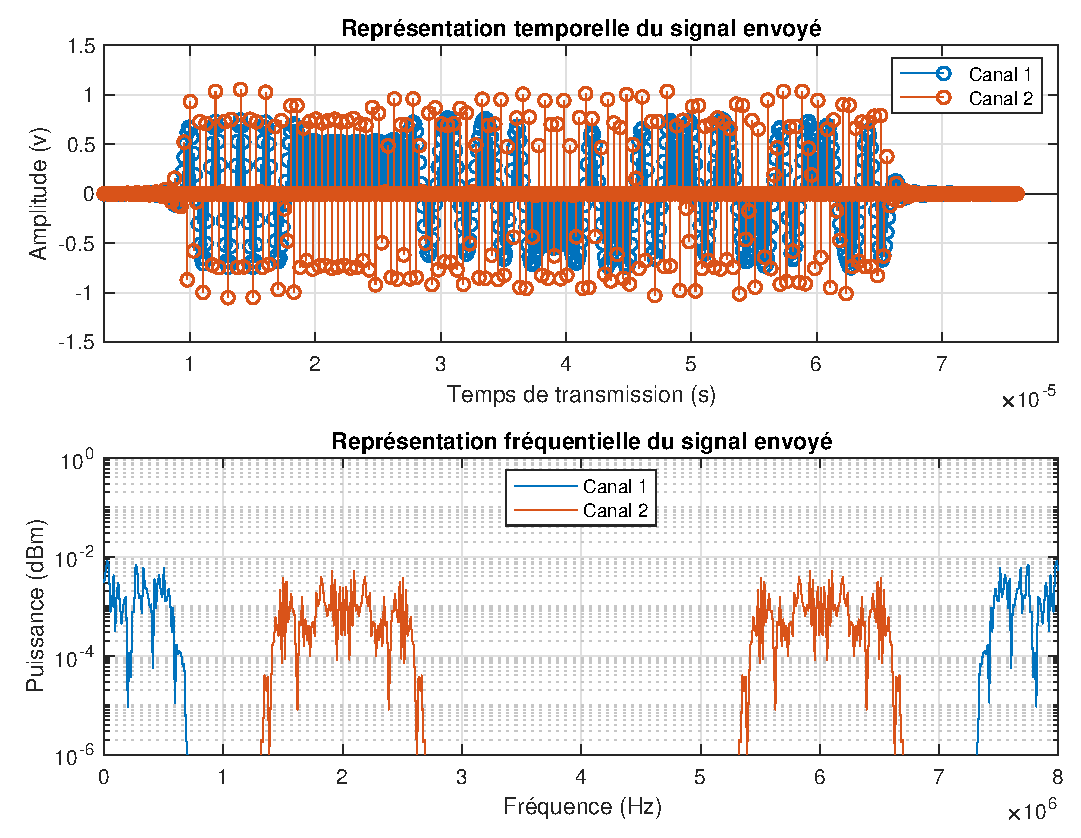
\includegraphics[height=0.4\textheight]{eps/sender.eps}
    \caption{Signaux de 50 bits chacun envoyés sur 2 canaux fréquentiels au rythme de 10 bit/s
             avec une fréquence d'échantillonage de \SI{80}{\hertz}.}
    \label{fig:sender}
\end{figure}

\subsection{Canal}
Le fichier \texttt{canal.m}, consultable à l'annexe~\ref{app:channel}, à pour mission de simuler les effets du canal de communication.
Nous nous attendons à ce qu'il se comporte comme un filtre passe-bas, c.-à-d. une atténuation des amplitudes et un décalage temporel.
Tout cela accompagné de bruit parasite.

Nous nous attendons à ce que le bruit soit de type AWGN, Additive White Gaussian Noise, pouvant être symbolisé par une variable aléatoire de distribution normale et de moyenne nulle $g[k]\sim\mathcal{N}(0,\sigma^2)$.
Tout commence par la génération d'un vecteur aléatoire de distribution normale de même taille que le vecteur de données.
Ce vecteur aléatoire est ensuite filtré pour ne pas contenir de fréquences supérieures à celle de Nyquist.
L'intensité du bruit se règle en multipliant le vecteur obtenu, qui est de variance 1, par l'écart-type liée à la variance désirée.
Un facteur d'atténuation A borné tel que $\num{0.6} \leq A \leq \num{0.9}$ est également généré.
Le script effectue ensuite $S_2[k] = A \cdot S_1[k] + g[k]$ pour appliquer l'atténuation et le bruit.
Du \og{}zero-padding\fg{} est ajouté au début du signal pour simuler un décalage temporel.

\subsection{Receveur}
Le fichier \texttt{receiver.m}, consultable à l'annexe~\ref{app:receiver}, se charge de ramener les signaux transmis en bande de base et prend des décisions sur les valeurs mesurées à tous les $T_b$ instants en espérant retrouver le signal original.

\subsubsection{Filtrage}
Le script commence par générer des filtres de type Butterworth qui vont lui permettre de séparer les canaux.
Pour filtrer, on commence par obtenir la fraction polynomiale représentant le filtre analogique.
De cette fonction, on calcule la réponse fréquentielle entre la fréquence 0 et la fréquence d'échantillonnage.
On applique la transformée de Fourier inverse à cette réponse fréquentielle, et nous obtenons la réponse impulsionnelle du filtre.
Il suffit dès lors de convoluer les échantillons temporels de notre signal avec les réponses impulsionnelles calculées et nous séparons ainsi les bandes spectrales.
Nous calculons des filtres d'ordre 10, la figure~\ref{fig:filters} et \ref{fig:grpdelay} présentent les filtres permettant de séparer les deux canaux utilisés dans cette simulation.

\subsubsection{Démodulation}
Une fois les canaux séparés, il faut les ramener en bande de base.
On ne peut pas simplement diviser les signaux pas un cosinus de même fréquence que la porteuse car le déphasage entre les deux laisserait une composante sinusoïdale parasite dans nos échantillons démodulés.
Pour obtenir notre signal en bande de base, nous multiplions encore le signal modulé avec un cosinus à même fréquence, multiplier deux cosinus amène à additionner leur fréquence.
Nous filtrons ensuite ce signal doublement multiplié par un filtre passe-bas pour supprimer les porteuses envoyées dans de plus hautes fréquences, et les fréquences restantes sont notre signal en bande de base.
En procédant de cette manière, nous contournons le problème d'estimation de la phase de la porteuse.

\begin{figure}[p]
    \centering
    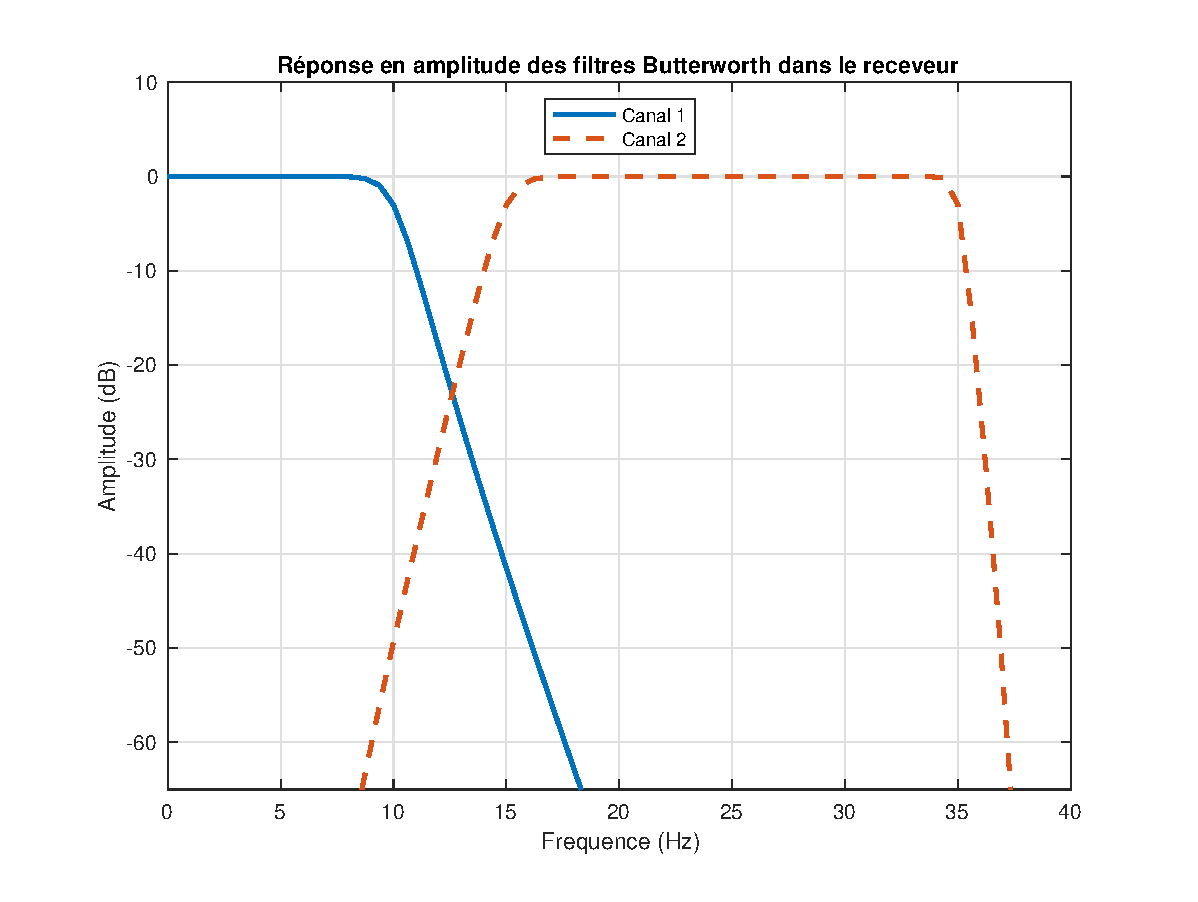
\includegraphics[height=0.4\textheight]{eps/filters.eps}
    \caption{Réponse en amplitude des filtres de type Butterworth utilisés dans le receveur
             pour séparer les canaux.
             Leurs pentes se rencontrent à \SI{-3}{\decibel}.}
    \label{fig:filters}
\end{figure}

\begin{figure}[p]
    \centering
    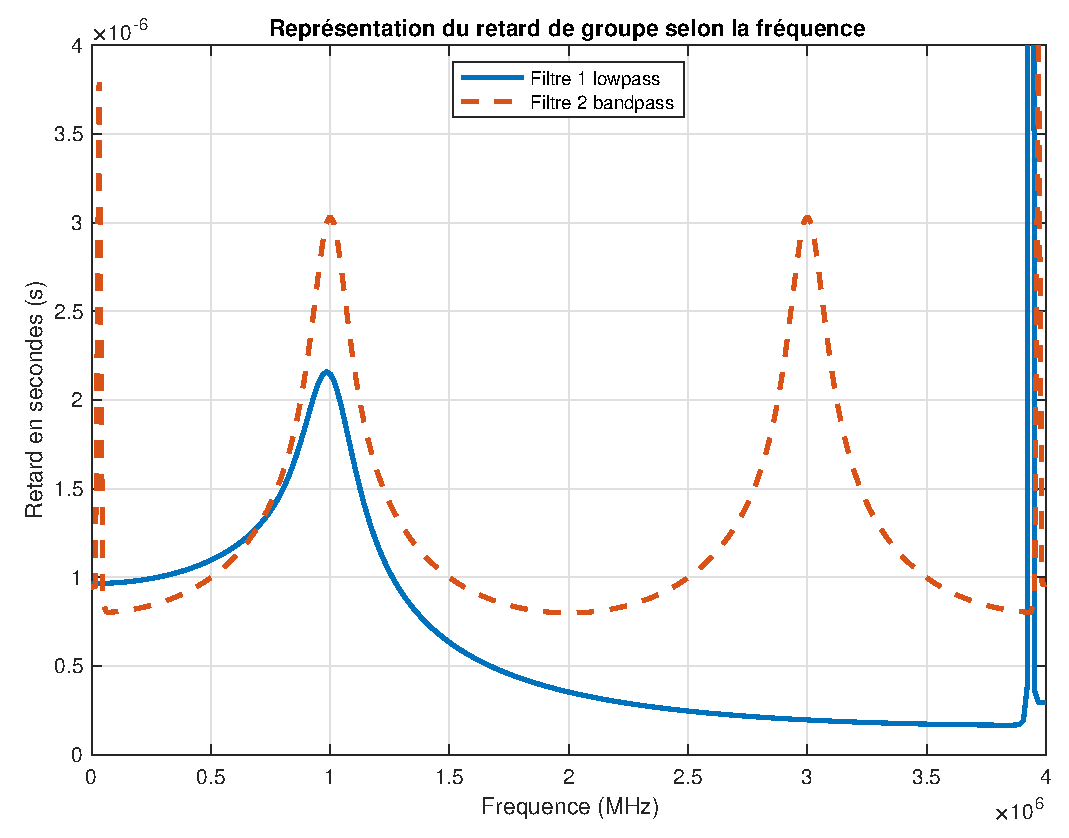
\includegraphics[height=0.4\textheight]{eps/grpdelay.eps}
    \caption{Retard de groupe des filtres de type Butterworth utilisés dans le receveur
             pour séparer les canaux.
             Le filtre 1 est un passe-bas avec une fréquence de coupure à \SI{1}{\mega\hertz}.
             Le filtre 2 est un passe-bande avec une fréquence de coupure basse à
             \SI{1}{\mega\hertz} et fréquence de coupure haute à \SI{3}{\mega\hertz}.
             Le filtre 2 est d'un degré double par rapport au 1 pour obtenir une pente
             semblable en amplitude. Cela se ressent dans le retard de groupe par une
             augmentation.}
    \label{fig:grpdelay}
\end{figure}

\subsubsection{Comparaison}
Le script receveur affiche un récapitulatif de la transmission reçue, comme l'émetteur affiche une récapitulatif de la transmission envoyée.
Ces récapitulatifs permettent de comparer les signaux émis avant d'être sommés dans l'environnement de transmission, \textit{e.g.} un câble, et les signaux reçus après les avoir séparés par filtrage.
La figure~\ref{fig:receiver} du receveur doit être comparée avec la figure~\ref{fig:sender} de l'émetteur.
On peut constater que : temporellement le receveur a un message décalé de quelques échantillons ; et fréquentiellement un signal atténué de quelques dBm.

\begin{figure}[p]
    \centering
    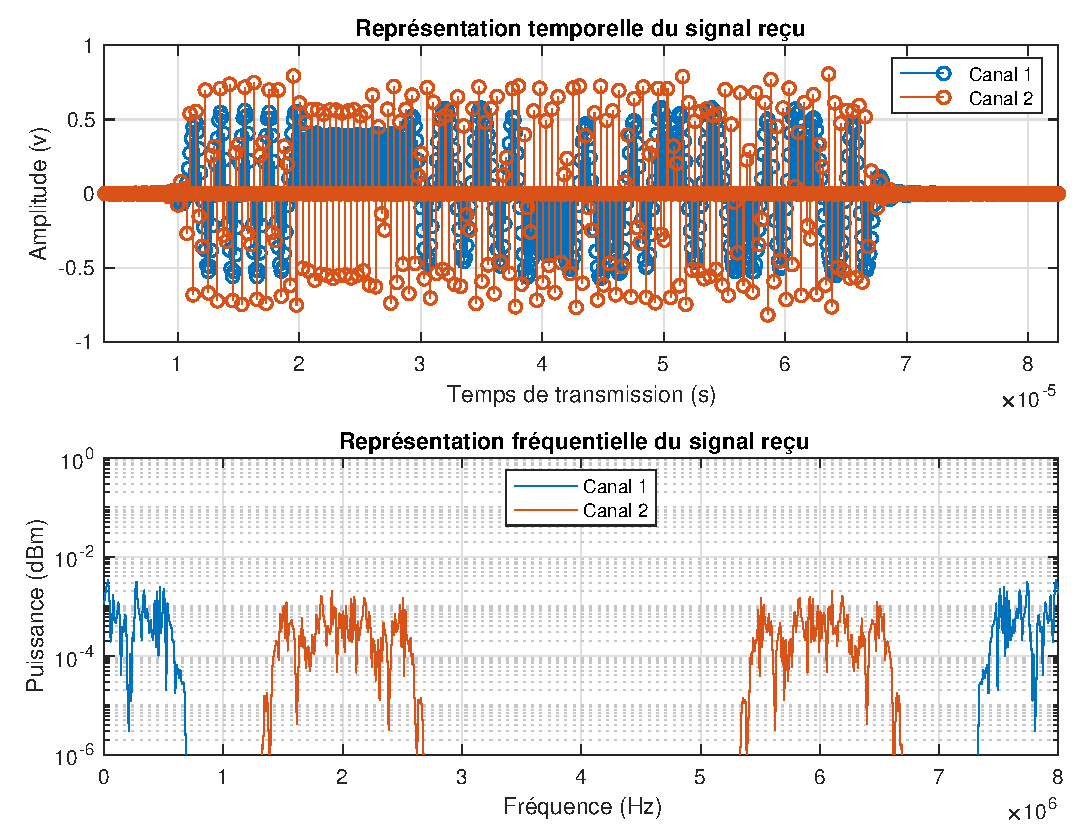
\includegraphics[height=0.4\textheight]{eps/receiver.eps}
    \caption{Signaux de 50 bits chacun envoyés sur 2 canaux fréquentiels au rythme de 10 bit/s
             avec une fréquence d'échantillonage de \SI{80}{\hertz}.}
    \label{fig:receiver}
\end{figure}

Une fois le signal en bande de base recomposé, le receveur doit repérer le début du signal et capturer un échantillon tous les $T_b$ instant.
Depuis cet échantillon capturé, il doit prendre la décision de choisir si le code transmis était $+1$ ou $-1$.
La simulation se permet de calculer le délai généré pour savoir où le signal commence.
Ceci est possible car nous disposons des réponses en phase de chaque filtre appliqué tout au long des calculs.
La figure~\ref{fig:decimate} présente un exemple de capture d'échantillons effectuée par le receveur.

\begin{figure}[p]
    \centering
    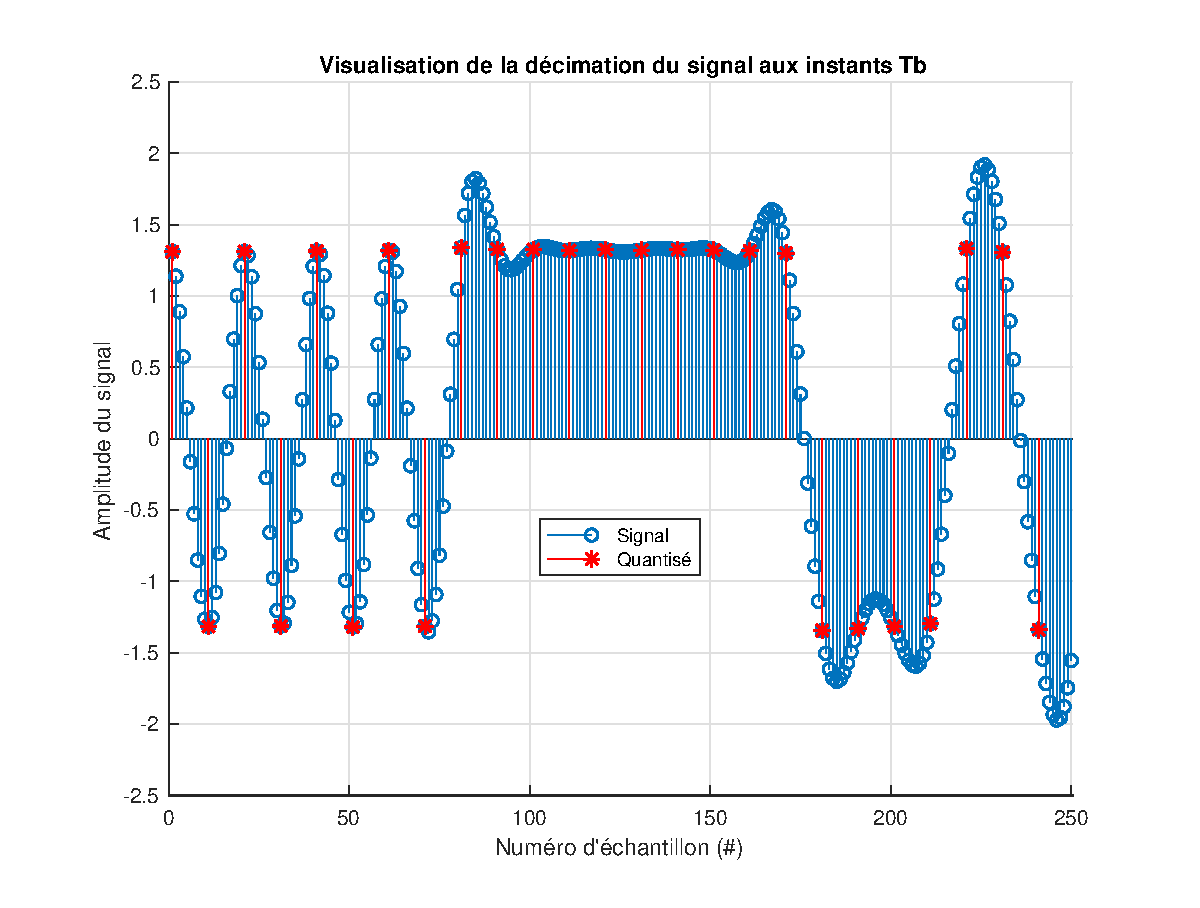
\includegraphics[height=0.4\textheight]{eps/decimate.eps}
    \caption{Visualisation de la capture d'échantillons pour le décideur.}
    \label{fig:decimate}
\end{figure}


\clearpage
%%%%%%%%%%%%%%%%%%%%%%
\section{Performances}
Dans le cas d'un code PAM-2, la relation $E_b/N_0$ au SNR s'écrit
\footnote{\url{https://nl.mathworks.com/help/comm/ug/awgn-channel.html}}
\begin{align}
    \frac{E_b}{N_0} + 10\log_{10}\left(\frac{R_b}{B}\right) = \text{SNR}_\text{dB}
\end{align}
Où sont définies les variables
\begin{description}[font=\rm,itemindent=1em,labelwidth=2em]
    \item[$E_b$] l'énergie d'un bit
    \item[$N_0$] la puissance du bruit pour un spectre partant de 0 à l'infini
    \item[$R_b$] le taux  de transmission des bits
    \item[$B$] la largueur de bande utilisée
    \item[SNR] le rapport de puissance $P_{\text{signal}}/
        P_{\text{noise}}$ en decibels
\end{description}
Puisque dans notre cas $R_b = B$, cela implique que $\log_{10}(R_b/B) = 0$, et nous pouvons l'ôter de l'équation pour ne laisser que la relation
\begin{equation}
    \frac{E_b}{N_0} = \text{SNR}_\text{dB}
    \label{eqn:ebn0-snr}
\end{equation}
Cette relation nous facilite grandement le calcul de $E_b/N_0$, nécessaire pour réaliser un diagramme BER.

Le diagramme BER, ou diagramme Bit-Error-Rate, est un digramme présentant le rapport du nombre de bits erronés reçus dans un intervalle de temps étudié, en fonction du rapport d'énergie d'un bit sur le bruit $E_b/N_0$.
Pour dessiner ce diagramme, nous désirons fixer un $E_b/N_0$ en abscisse, et reporter son taux d'erreur en ordonnée.
Mais encore faut-il savoir fixer un $E_b/N_0$.
C'est ici que l'équation~(\ref{eqn:ebn0-snr}) vient grandement nous aider car elle nous permet de fixer un $E_b/N_0$ en modifiant l'amplitude du bruit simulé.
\begin{gather}
    \intertext{Depuis la formule du SNR qui \underline{n'est pas} exprimée en decibels}
    \text{SNR} = \frac{P_\text{signal}}{P_\text{noise}}
        = \frac{\sum_{n=0}^{N}\text{signal}[n]^2}{\sum_{n=0}^{N}\text{noise}[n]^2}
    \intertext{Et connaissant le rapport de puissance que nous souhaitons obtenir}
    10^{\left(\text{dB}/10\right)} = \text{SNR}
    \intertext{Nous pouvons calculer un ratio qui nous amène au niveau de bruit désiré}
    \text{ratio} = \frac{\text{SNR}}{10^{\left(\text{dB}/10\right)}}
    \intertext{Et nous normalisons le bruit en le multipliant par la racine de ce ratio pour arriver au SNR voulu}
    \text{noise leveled} = \text{noise} \times \sqrt{\text{ratio}}
\end{gather}
Cette operation s'effectue dans le fichier \texttt{channel.m}.

Nous pouvons dès lors tracer le diagramme BER de notre méthode de transmission en lui adjoignant le BER mathématiquement optimal d'une modulation PAM-2 défini par l'équation~\ref{eqn:best-ber}. Cette relation est donnée et acceptée.
\begin{equation}
    \text{BER}_\text{PAM-2} = \frac{1}{2}\,\text{erfc}\left(\sqrt{\frac{E_b}{N_0}}\right)
    \label{eqn:best-ber}
\end{equation}
\begin{figure}[!ht]
    \centering
    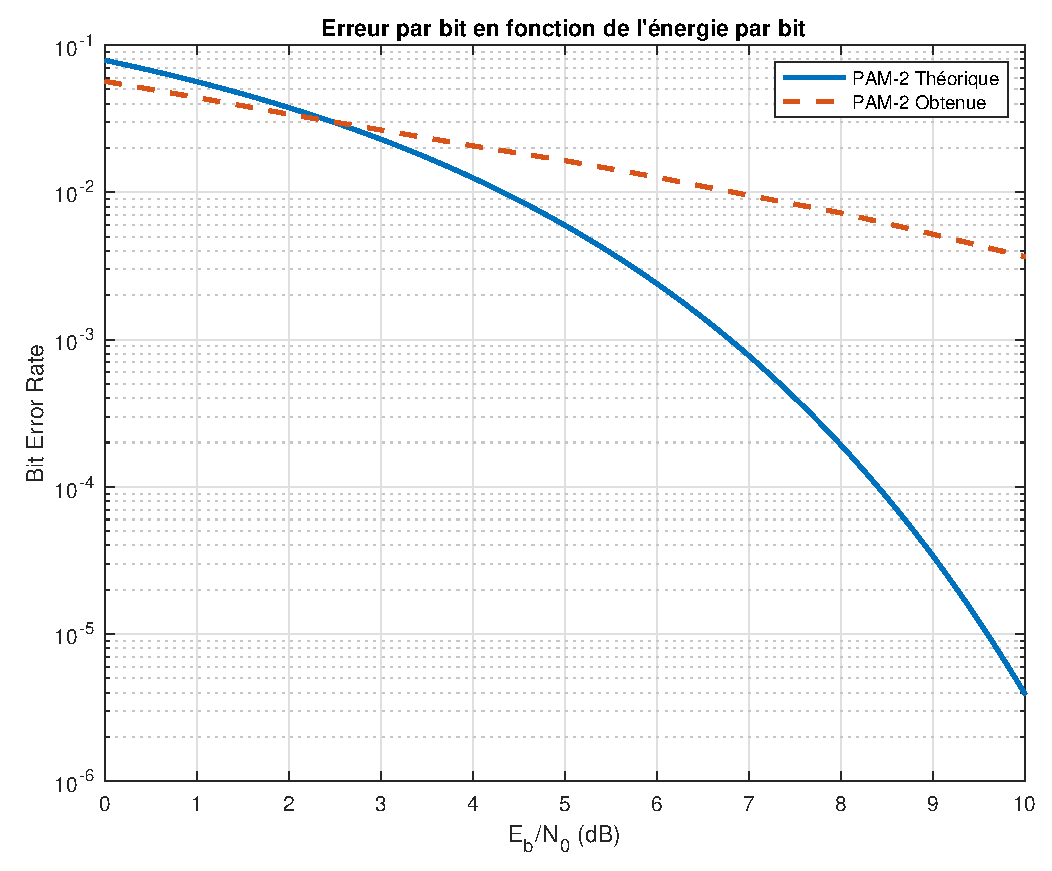
\includegraphics[height=0.4\textheight]{eps/ber-curve.eps}
    \caption{Courbe du taux d'erreur par bit BER en fonction de l'énergie par bit
             $E_b/N_0$, aussi appelé SNR par bit.
             La figure reprend la courbe optimale mathématiquement et la courbe évaluée
             grâce à MATLAB. La courbe évaluée se comporte étonnement en faisant mieux
             que l'optimum théorique avant \SI{2.5}{\decibel} et pire après.}
    \label{fig:ber-curve}
\end{figure}
La figure~\ref{fig:ber-curve} présente le diagramme BER mathématiquement optimal calculé depuis la fonction d'erreur~\ref{eqn:best-ber}, et le diagramme BER de notre projet évalué dans MATLAB.

%%%%%%%%%%%%%%%
\phantomsection
\section*{Conclusion}
\addcontentsline{toc}{section}{Conclusion}
À la fin du projet nous avons rencontré plusieurs comportements non attendus.
Le premier est le gain en tension du premier canal fréquentiel survenant après démodulation dans le récepteur.
Cet effet est constatable à la figure~\ref{fig:comparaison}.
Ce gain pourrait venir du filtrage.

Un second problème vient de la modulation des impulsions de mise en forme.
Multiplier par certaines fréquences a pour effet que le signal est inversé au moment de l'échantillonnage.
Cet effet peut se voir sur la figure~\ref{fig:impulse} sur le canal 2.

Un troisième problème est la chute du taux d'erreur qui est beaucoup plus lente que prévue.
Cet effet peut se constater sur la figure~\ref{fig:ber-curve}.
Notre taux d'erreur est même supérieur à l'optimal mathématique avant \SI{2.5}{\decibel}.

Le dernier problème est apparu quand nous avons cherché à comprendre le 3\up{ème} problème.
Le taux d'erreur sur un canal varie selon le nombre de canaux actifs présents, et ce de manière arbitraire.
Le tableau~\ref{tab:ber-per-channel} présente des mesures que nous avons relevées.
On peut constater que le taux d'erreur dans le canal 1 baisse au fur et à mesure que nous rajoutons des canaux.

\begin{table}[!ht]
    \centering
    \begin{tabular}{l|llll}
    & \bf Canal 1 & \bf Canal 2 & \bf Canal 3 & \bf Canal 4\\
    \hline
    \bf 1 actif  & 0.4310 & n/a    & n/a    & n/a\\
    \bf 2 actifs & 0.4101 & 0.4456 & n/a    & n/a\\
    \bf 3 actifs & 0.3918 & 0.4706 & 0.4703 & n/a\\
    \bf 4 actifs & 0.3762 & 0.5279 & 0.4161 & 0.5271
    \end{tabular}
    \caption{Taux d'erreur moyen variant selon le nombre de canaux actifs.}
    \label{tab:ber-per-channel}
\end{table}

Malgré l'imperfection de notre simulation, nous parvenons à transmettre plusieurs signaux avec des taux d'erreurs relativement faible pour un SNR réaliste supérieur à \SI{10}{\decibel}.

%%%%%%%%%
\appendix
\clearpage

\section{Figures arbitraires}
\label{sec:uncommented-figure}

\begin{figure}[!h]
    \centering
    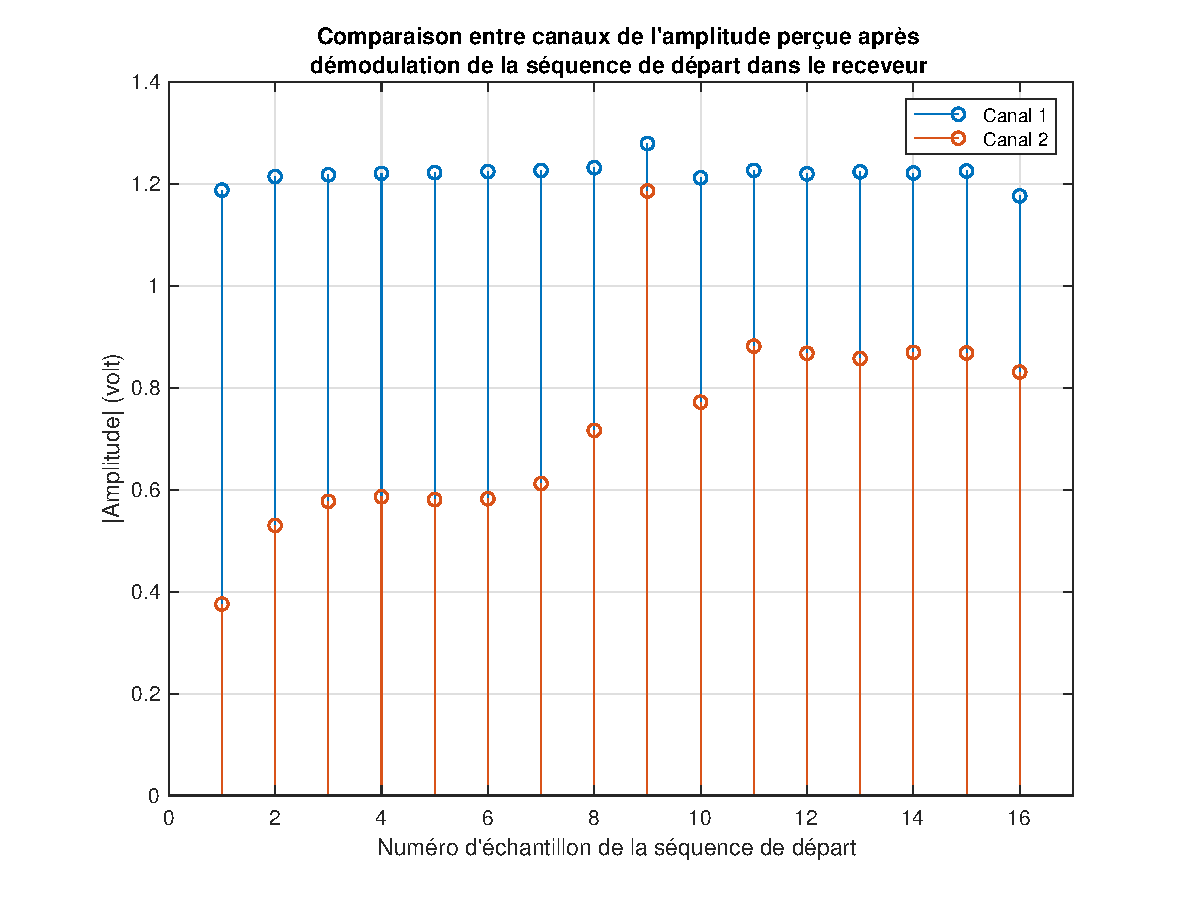
\includegraphics[height=0.4\textheight]{eps/startSeq-comparaison.eps}
    \caption{Atténuation de l'amplitude de la séquence de départ perçue
             dans le receveur.
             Si l'amplitude de la séquence du premier canal reste constante après
             transmission, cela n'est pas du tout vrai pour le second où la perte
             de tension n'est pas homogène.
             Ce défaut nous a empêché d'implémenter un mécanisme de normalisation
             à l'entrée du receveur basé sur la séquence de départ.}
\end{figure}
\vfill
\begin{figure}[!h]
    \centering
    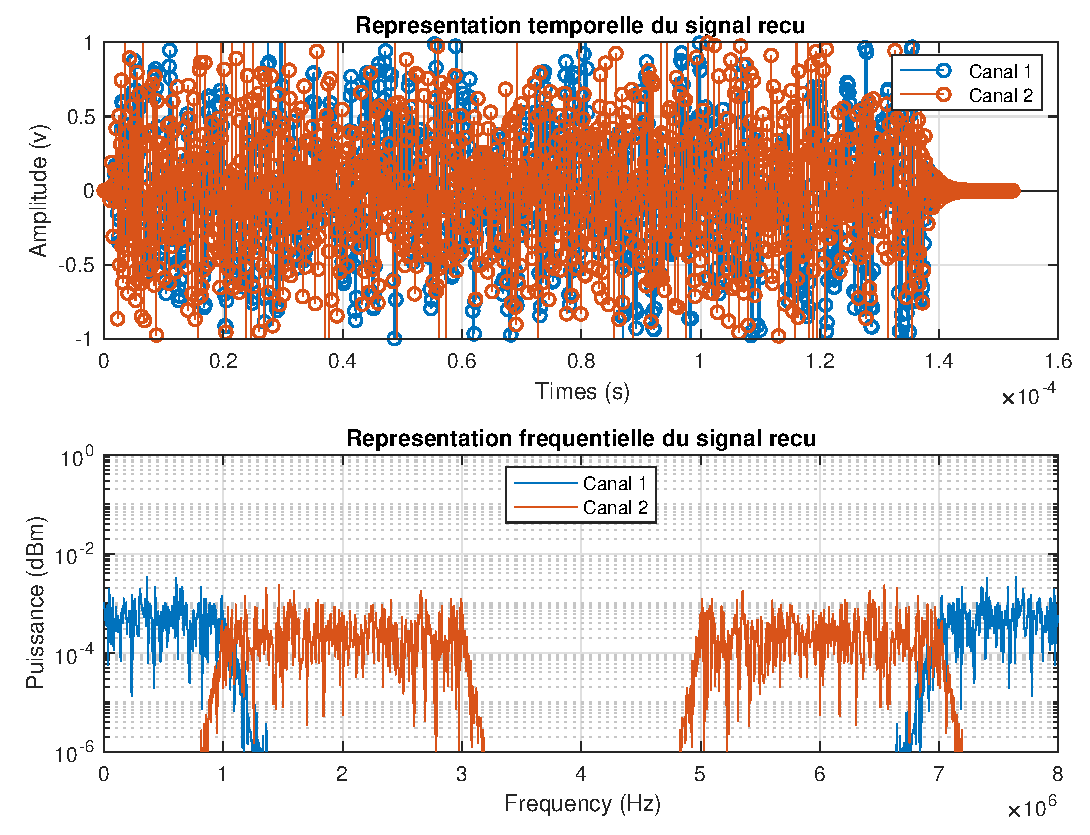
\includegraphics[height=0.35\textheight]{eps/noised.eps}
    \caption{Sortie des filtres dans le receveur servant à séparer les canaux
             fréquentiels, dans le cas d'un signal fortement bruité.
             Cette figure permet de montrer les limites de bande passante des
             filtres.}
\end{figure}
% second page
\begin{figure}[!ht]
    \centering
    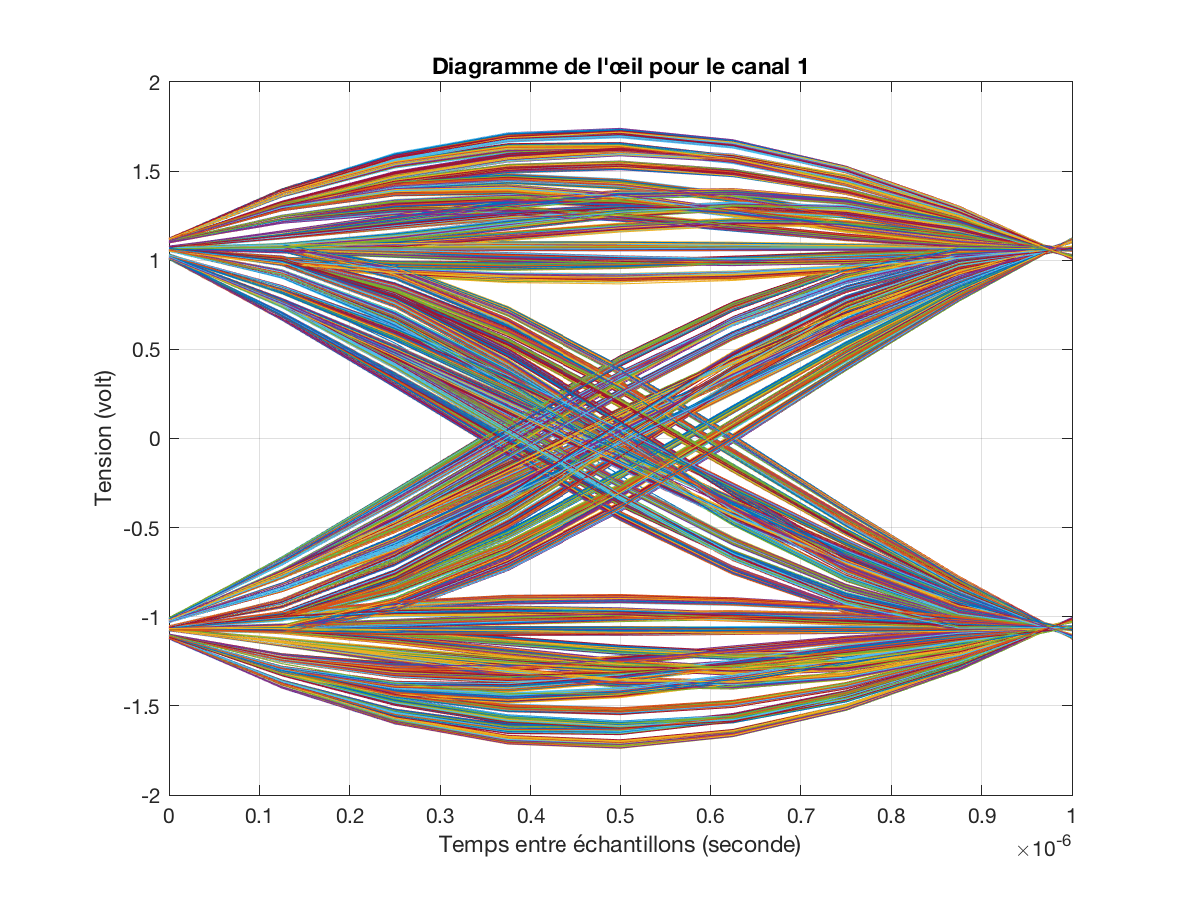
\includegraphics[height=0.4\textheight]{eps/eyediagram1.eps}
    \caption{Diagramme de l'œil pour le canal 1 sans bruit ajouté.
             On constate que les transitions ne sont pas homogènes malgré l'absence
             du bruit de canal.}
\end{figure}
\vfill
\begin{figure}[!ht]
    \centering
    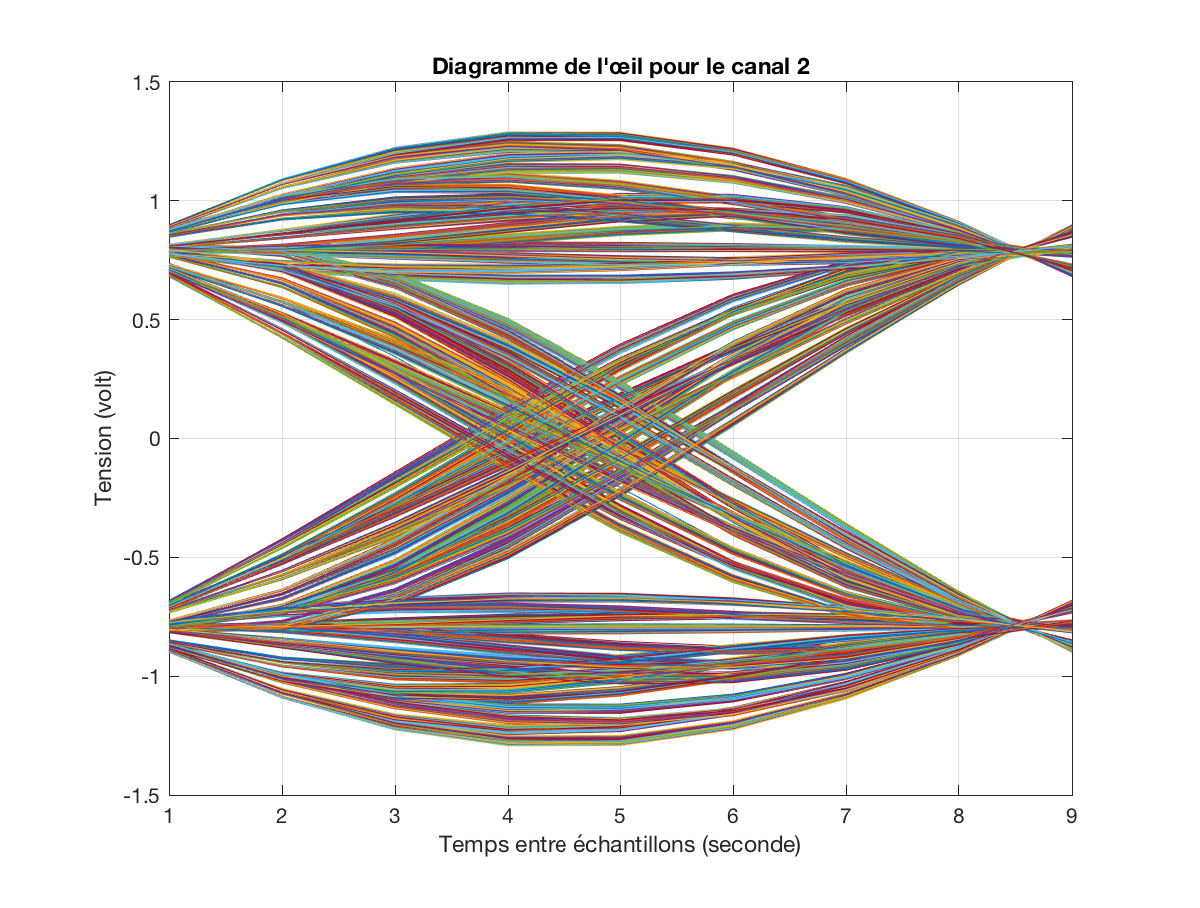
\includegraphics[height=0.4\textheight]{eps/eyediagram2.eps}
    \caption{Diagramme de l'œil pour le canal 2 sans bruit ajouté.
             On constate que les transitions ne sont pas homogènes malgré l'absence
             du bruit de canal.}
\end{figure}

\clearpage

\section{Fichiers sources}
\label{sec:fichiers-sources}

\subsection{main.m}
\inputminted{matlab}{../main.m}
\label{app:main}

\subsection{parameters.m}
\inputminted{matlab}{../parameters.m}
\label{app:paremeters}

\subsection{sender.m}
\inputminted{matlab}{../sender.m}
\label{app:sender}

\subsection{channel.m}
\inputminted{matlab}{../channel.m}
\label{app:channel}

\subsection{receiver.m}
\inputminted{matlab}{../receiver.m}
\label{app:receiver}

\subsection{filters.m}
\inputminted{matlab}{../filters.m}
\label{app:filters}

\subsection{diagram.m}
\inputminted{matlab}{../diagram.m}
\label{app:diagram}

\end{document}
